\section{Open questions}\label{sec:open}
Each problem states the nearest proved theorem and the missing obligation. Problems already settled by the cited releases are not repeated.
\begin{description}[leftmargin=1.2em,itemsep=3pt]
\item[O1. Classification of history complexes.] \emph{Nearest:} the fixed-content classification of $\{2,3,14\}$ (\Src{II}{thm:2314}) and the scoped block rewrites (\Src{II}{thm:block}). \emph{Missing:} a classification of swap classes and route homology for arbitrary content and source.
\item[O2. Reconstruction of ancestry from richer invariants.] \emph{Nearest:} faithfulness of the fibre sequence (\cref{thm:faith-cited}) and the obstruction \cref{prop:P5}. \emph{Missing:} a characterisation of the invariants of an endpoint, strictly between $D(t)$ and the whole fibre sequence, that determine the number of histories or of classes.
\item[O3. Maps between the two geometries.] \emph{Question:} maps between history geometry and evolving occurrence geometry, and non-identity intertwining of the two dynamics. \emph{Nearest:} the translation formula \cref{prop:P9}(c) and the restricted event correspondences \Src{III}{thm:B2T10}, \Src{III}{thm:R3T7}. \emph{Missing:} a map at level L3 or L4 beyond the rigid domain and the listed pairs, and either a construction or a non-existence proof for a non-identity $\Phi$ with $\Phi\circ C=T\circ\Phi$ (the obstruction \cref{prop:P9}(a) excludes only $\Phi=\mathrm{id}$).
\item[O4. Prediction of higher-dimensional Betti changes.] \emph{Nearest:} \cref{prop:P7}(c) and the zig-zag identity. \emph{Missing:} determination of $\Delta\beta_i$, $i\ge1$, when $2$-cells are present, from data cheaper than the full target.
\item[O5. Effective onset and closed Betti laws for towers.] \emph{Nearest:} \Src{III}{thm:A5T53} (qualitative quasi-polynomials) and \Src{III}{thm:A5T6} (exact to $k\le140$), \cref{prop:P8}. \emph{Missing:} an effective threshold, exact formulas for all $k$, and an invariant of $S_0$ that governs the Betti vector.
\item[O6. Reachability of activation families.] \emph{Nearest:} \Src{III}{thm:A4T1} and \Src{III}{thm:A5T24}. \emph{Missing:} a complete arithmetic classification of the families that occur along actual orbits.
\item[O7. Transition laws for dormant primitive systems.] \emph{Nearest:} \Src{I}{thm:P2T2}, \cref{lem:minimal}, \cref{cor:S4}. \emph{Missing:} an identification of the order on lattice vectors with the divisor-interval order on pairs of occurrences under compatible hypotheses, or an obstruction to one.
\item[O8. Compatibility of arithmetic guards.] \emph{Nearest:} the bijection \cref{prop:P2}(a) at the level of integers. \emph{Missing:} an extension of the generative rule to rational sources whose predecessor guard reproduces $d\equiv1\pmod b$.
\end{description}

\noindent\Cref{fig:frontier} shows established conclusions and open construction obligations.

\begin{figure}[t]\centering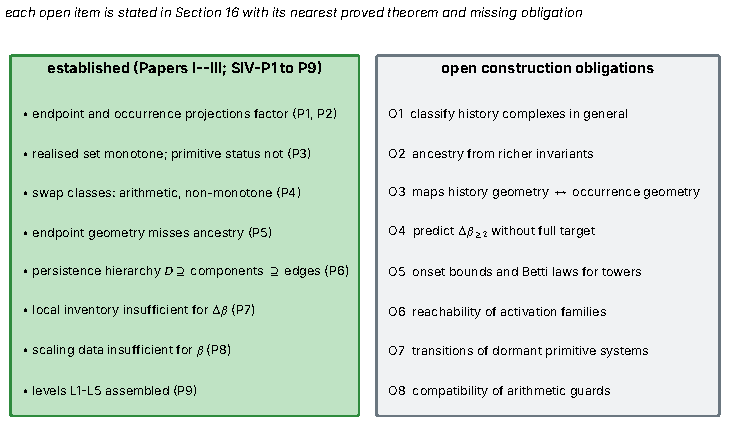
\includegraphics[width=\linewidth]{fig22_conclusions_open.pdf}
\caption{\textbf{Established conclusions and open construction obligations.} Left: the nine propositions; right: the eight open problems of this section. \emph{Schematic summary; each item is defined and referenced in the text.}}\label{fig:frontier}\end{figure}

\subsection{Operational versus intrinsic characterisation}\label{sec:intrinsic}
\Cref{sec:characterisation} characterises the Substrate \emph{operationally}: through the operators, domains, routes and admissibility conditions that are actually used, and the proved relations among the structures they generate. An \emph{intrinsic} characterisation would instead derive these components, and the associated constructions, from a minimal list of axioms and show which of them are independent. The two are different mathematical problems, and only the first is addressed here. \emph{Nearest proved results:} the factorizations and obstructions of \cref{prop:P1,prop:P2,prop:P5} and the status map of \cref{fig:global}. \emph{Missing obligations:}
\begin{enumerate}[label=(\roman*),itemsep=1pt]
\item an axiomatic definition of admissibility from which the guards $N\mid m$ and $d^2\mid a$, $d\equiv1\ (b)$ both follow (the identification is proved only for integer states, \cref{prop:P2}(a); see O8);
\item a compatibility statement placing $T_N$ and $C$ in one admissibility system, or a proof that no non-identity intertwining exists (O3);
\item a proof that the associated constructions (occurrence set, relation lattice, primitive system, complex) are determined by, or independent of, the schematic components $(S,\mathcal O,\mathrm{Dom},\mathcal R,\mathsf{Adm})$, rather than assumed through definitions;
\item the passage from the finite-exact ranges recorded here to statements for all sources, which no result of this paper provides.
\end{enumerate}
